\documentclass[border=4pt]{standalone}
\usepackage{amsmath,amssymb,tikz}
\usetikzlibrary{arrows.meta}
\definecolor{figB}{RGB}{31,90,166}\definecolor{figR}{RGB}{176,48,48}\definecolor{figG}{RGB}{60,130,60}
\begin{document}
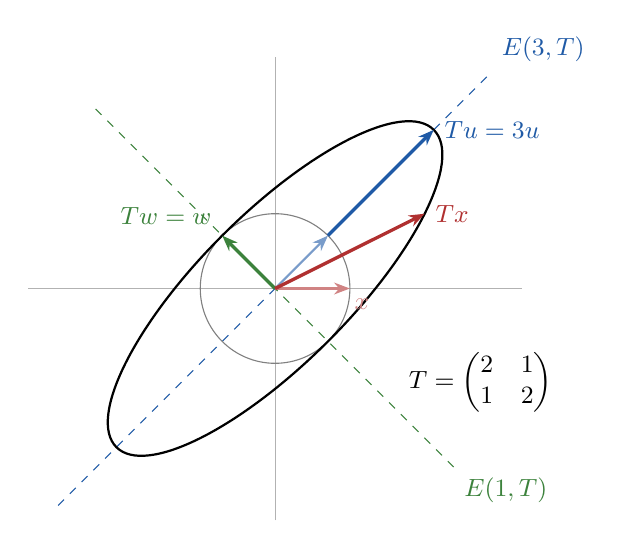
\begin{tikzpicture}[scale=0.95,>={Stealth[length=2mm]}]
\draw[gray!60] (-3.3,0)--(3.3,0); \draw[gray!60] (0,-3.1)--(0,3.1);
\draw[dashed,figB] (-2.9,-2.9)--(2.9,2.9) node[above right,font=\small]{$E(3,T)$};
\draw[dashed,figG] (-2.4,2.4)--(2.4,-2.4) node[below right,font=\small]{$E(1,T)$};
\draw[gray] (0,0) circle (1);
\draw[black,thick,rotate=45] (0,0) ellipse (3 and 1);
\draw[->,thick,figB!60] (0,0)--(0.707,0.707);
\draw[->,very thick,figB] (0.707,0.707)--(2.121,2.121) node[right,font=\small]{$Tu=3u$};
\draw[->,very thick,figG] (0,0)--(-0.707,0.707) node[above left,font=\small]{$Tw=w$};
\draw[->,thick,figR!60] (0,0)--(1,0) node[below right,font=\small,xshift=-2pt]{$x$};
\draw[->,very thick,figR] (0,0)--(2,1) node[right,font=\small]{$Tx$};
\node[font=\small] at (2.75,-1.25) {$T=\begin{pmatrix}2&1\\1&2\end{pmatrix}$};
\end{tikzpicture}
\end{document}
